\documentclass[11pt,oneside]{article}
\pdfminorversion=7
\usepackage{QuizStyle}
\hypersetup{
    pdftitle={20260915 Quiz for MATH230 Probability \& Statistics},
    pdfauthor={Jungwoo Kim},
    pdfsubject={Quiz for MATH230 Probability \& Statistics},
    pdfcreator={LaTeX}
}
\begin{document}
\quiztitle{20260915 Quiz}
\begin{exercise}{2.5}
A die is tossed. If the result is even, a coin is flipped once; if the result is odd, the coin is flipped twice. For example, $4H$ denotes a 4 followed by a head, and $3HT$ denotes a 3 followed by a head and a tail. Draw a tree diagram displaying the 18 outcomes in the sample space $S$.
\end{exercise}

\begin{solution}
The six die results determine the first branches. Even outcomes have two possible coin sequences; odd outcomes have four. The complete tree is
\begin{center}
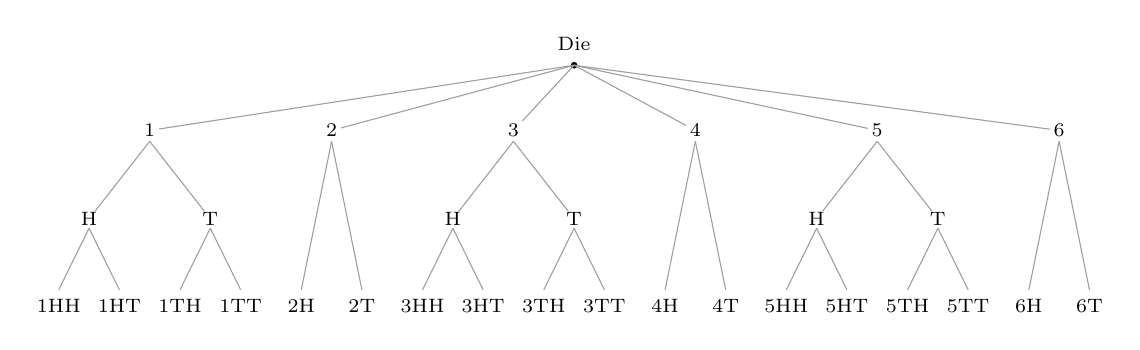
\begin{tikzpicture}[x=0.77cm,y=0.92cm, every node/.style={font=\scriptsize}]
\node at (8.5,3.8) {Die};
\fill (8.5,3.5) circle (1.2pt);
\draw[gray!75] (8.5,3.5)--(1.5,2.6);
\node[fill=white,inner sep=1.3pt] at (1.5,2.6) {1};
\draw[gray!75] (1.5,2.45)--(0.5,1.38);
\node[fill=white,inner sep=0.5pt] at (0.5,1.38) {H};
\draw[gray!75] (0.5,1.25)--(0,0.4);
\node[below] at (0,0.4) {1HH};
\draw[gray!75] (0.5,1.25)--(1,0.4);
\node[below] at (1,0.4) {1HT};
\draw[gray!75] (1.5,2.45)--(2.5,1.38);
\node[fill=white,inner sep=0.5pt] at (2.5,1.38) {T};
\draw[gray!75] (2.5,1.25)--(2,0.4);
\node[below] at (2,0.4) {1TH};
\draw[gray!75] (2.5,1.25)--(3,0.4);
\node[below] at (3,0.4) {1TT};
\draw[gray!75] (8.5,3.5)--(4.5,2.6);
\node[fill=white,inner sep=1.3pt] at (4.5,2.6) {2};
\draw[gray!75] (4.5,2.45)--(4,0.4);
\node[below] at (4,0.4) {2H};
\draw[gray!75] (4.5,2.45)--(5,0.4);
\node[below] at (5,0.4) {2T};
\draw[gray!75] (8.5,3.5)--(7.5,2.6);
\node[fill=white,inner sep=1.3pt] at (7.5,2.6) {3};
\draw[gray!75] (7.5,2.45)--(6.5,1.38);
\node[fill=white,inner sep=0.5pt] at (6.5,1.38) {H};
\draw[gray!75] (6.5,1.25)--(6,0.4);
\node[below] at (6,0.4) {3HH};
\draw[gray!75] (6.5,1.25)--(7,0.4);
\node[below] at (7,0.4) {3HT};
\draw[gray!75] (7.5,2.45)--(8.5,1.38);
\node[fill=white,inner sep=0.5pt] at (8.5,1.38) {T};
\draw[gray!75] (8.5,1.25)--(8,0.4);
\node[below] at (8,0.4) {3TH};
\draw[gray!75] (8.5,1.25)--(9,0.4);
\node[below] at (9,0.4) {3TT};
\draw[gray!75] (8.5,3.5)--(10.5,2.6);
\node[fill=white,inner sep=1.3pt] at (10.5,2.6) {4};
\draw[gray!75] (10.5,2.45)--(10,0.4);
\node[below] at (10,0.4) {4H};
\draw[gray!75] (10.5,2.45)--(11,0.4);
\node[below] at (11,0.4) {4T};
\draw[gray!75] (8.5,3.5)--(13.5,2.6);
\node[fill=white,inner sep=1.3pt] at (13.5,2.6) {5};
\draw[gray!75] (13.5,2.45)--(12.5,1.38);
\node[fill=white,inner sep=0.5pt] at (12.5,1.38) {H};
\draw[gray!75] (12.5,1.25)--(12,0.4);
\node[below] at (12,0.4) {5HH};
\draw[gray!75] (12.5,1.25)--(13,0.4);
\node[below] at (13,0.4) {5HT};
\draw[gray!75] (13.5,2.45)--(14.5,1.38);
\node[fill=white,inner sep=0.5pt] at (14.5,1.38) {T};
\draw[gray!75] (14.5,1.25)--(14,0.4);
\node[below] at (14,0.4) {5TH};
\draw[gray!75] (14.5,1.25)--(15,0.4);
\node[below] at (15,0.4) {5TT};
\draw[gray!75] (8.5,3.5)--(16.5,2.6);
\node[fill=white,inner sep=1.3pt] at (16.5,2.6) {6};
\draw[gray!75] (16.5,2.45)--(16,0.4);
\node[below] at (16,0.4) {6H};
\draw[gray!75] (16.5,2.45)--(17,0.4);
\node[below] at (17,0.4) {6T};
\end{tikzpicture}
\end{center}
Hence $|S|=3(2)+3(4)=\boxed{18}$.
\end{solution}

\begin{exercise}{2.9}
In the die-and-coin experiment, the die is tossed first. After an even result the coin is flipped once; after an odd result it is flipped twice. List the elements of (a) the event $A$ that the die shows a number less than 3, (b) the event $B$ of two tails, and (c) the complement $A'$.
\end{exercise}

\begin{solution}
\begin{align*}
\textup{(a)}\quad A&=\{1HH,1HT,1TH,1TT,2H,2T\},\\
\textup{(b)}\quad B&=\{1TT,3TT,5TT\},\\
\textup{(c)}\quad A'&=\{3HH,3HT,3TH,3TT,4H,4T,5HH,5HT,5TH,5TT,6H,6T\}.
\end{align*}
\end{solution}

\Needspace{16\baselineskip}
\begin{exercise}{2.14}
Let $S=\{0,1,2,3,4,5,6,7,8,9\}$, $A=\{0,2,4,6,8\}$, $B=\{1,3,5,7,9\}$, $C=\{2,3,4,5\}$, and $D=\{1,6,7\}$. List the elements of
\par
\begin{exercisesubparts}
\item $A\cup D$
\item $A\cap B$
\item $B'$
\item $(B'\cap D)\cup A$
\item $(S\cap D)'$
\item $A\cap C\cap D'$
\end{exercisesubparts}
\end{exercise}

\begin{solution}
Taking complements relative to $S$ gives
\begin{align*}
\textup{(a)}&\ \boxed{\{0,1,2,4,6,7,8\}},\\
\textup{(b)}&\ \boxed{\varnothing},\\
\textup{(c)}&\ \boxed{\{0,2,4,6,8\}},\\
\textup{(d)}&\ \boxed{\{0,2,4,6,8\}},\\
\textup{(e)}&\ \boxed{\{0,2,3,4,5,8,9\}},\\
\textup{(f)}&\ \boxed{\{2,4\}}.
\end{align*}
\end{solution}

\begin{exercise}{2.16}
Let $S=\{x\in\mathbb R\mid 0<x<12\}$, $M=\{x\in S\mid1<x<8\}$, and $N=\{x\in S\mid0<x<6\}$. Find (a) $M\cup N$, (b) $M\cap N$, and (c) $M'\cap N'$ relative to $S$.
\end{exercise}

\begin{solution}
The union and intersection of the intervals give
\begin{align*}
\textup{(a)}&\quad\boxed{(0,8)},\\
\textup{(b)}&\quad\boxed{(1,6)},\\
\textup{(c)}&\quad\boxed{[8,12)}.
\end{align*}
\end{solution}

\begin{exercise}{2.19}
For a family on a camping vacation, let $M$ denote mechanical problems, $T$ a traffic ticket, and $V$ arrival at a campsite with no vacancies. Use the numbered regions in the diagram below.
\begin{center}
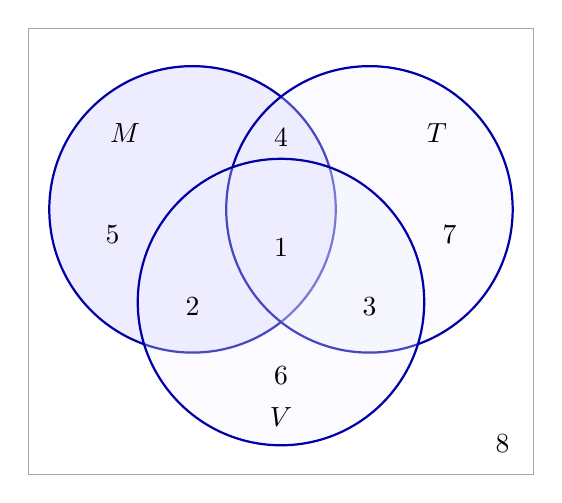
\begin{tikzpicture}[scale=1.07]
\draw[thin,gray!70] (-3,-2.8) rectangle (3,2.5);
\draw[thick,blue!65!black,fill=blue!7] (-1.05,0.35) circle (1.70);
\draw[thick,blue!65!black,fill=blue!7,fill opacity=0.30] (1.05,0.35) circle (1.70);
\draw[thick,blue!65!black,fill=blue!7,fill opacity=0.30] (0,-0.75) circle (1.70);
\node at (-1.85,1.25) {$M$}; \node at (1.85,1.25) {$T$};
\node at (0,-2.12) {$V$};
\node at (0,-0.10) {1}; \node at (-1.05,-0.80) {2};
\node at (1.05,-0.80) {3}; \node at (0,1.20) {4};
\node at (-2,0.05) {5}; \node at (0,-1.62) {6};
\node at (2,0.05) {7}; \node at (2.63,-2.43) {8};
\end{tikzpicture}
\end{center}

\par
\begin{exercisesubparts}
\item Describe region 5 in words.
\item Describe region 3 in words.
\item Describe regions 1 and 2 together.
\item Describe regions 4 and 7 together.
\item Describe regions 3, 6, 7, and 8 together.
\end{exercisesubparts}
\end{exercise}

\begin{solution}
The regions are, respectively,
\begin{exercisesubparts}
\item Mechanical problems, but neither a ticket nor a full campsite ($M\cap T'\cap V'$).
\item A ticket and a full campsite, but no mechanical problems ($M'\cap T\cap V$).
\item Mechanical problems and a full campsite, whether or not a ticket occurs ($M\cap V$).
\item A ticket but no full campsite, regardless of mechanical problems ($T\cap V'$).
\item No mechanical problems ($M'$).
\end{exercisesubparts}
\end{solution}

\begin{exercise}{2.20}
For a family on a camping vacation, let $M$ denote mechanical problems, $T$ a traffic ticket, and $V$ arrival at a campsite with no vacancies. Use the numbered regions in the diagram below.
\begin{center}
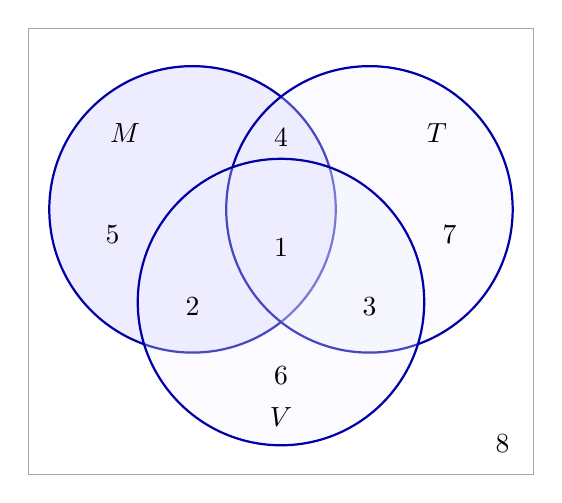
\begin{tikzpicture}[scale=1.07]
\draw[thin,gray!70] (-3,-2.8) rectangle (3,2.5);
\draw[thick,blue!65!black,fill=blue!7] (-1.05,0.35) circle (1.70);
\draw[thick,blue!65!black,fill=blue!7,fill opacity=0.30] (1.05,0.35) circle (1.70);
\draw[thick,blue!65!black,fill=blue!7,fill opacity=0.30] (0,-0.75) circle (1.70);
\node at (-1.85,1.25) {$M$}; \node at (1.85,1.25) {$T$};
\node at (0,-2.12) {$V$};
\node at (0,-0.10) {1}; \node at (-1.05,-0.80) {2};
\node at (1.05,-0.80) {3}; \node at (0,1.20) {4};
\node at (-2,0.05) {5}; \node at (0,-1.62) {6};
\node at (2,0.05) {7}; \node at (2.63,-2.43) {8};
\end{tikzpicture}
\end{center}

\par
\begin{exercisesubparts}
\item No mechanical problems and no ticket, but a campsite with no vacancies.
\item Mechanical problems and a full campsite, but no ticket.
\item Mechanical problems or a full campsite, but no ticket.
\item The family does not arrive at a full campsite.
\end{exercisesubparts}
\end{exercise}

\begin{solution}
Reading the labeled regions gives
\begin{align*}
\textup{(a)}&\quad\boxed{\{6\}},\\
\textup{(b)}&\quad\boxed{\{2\}},\\
\textup{(c)}&\quad\boxed{\{2,5,6\}},\\
\textup{(d)}&\quad\boxed{\{4,5,7,8\}}.
\end{align*}
\end{solution}

\begin{exercise}{2.22}
A patient is classified by blood type and blood-pressure category. The eight blood types are
\[
AB^+,\ AB^-,\ A^+,\ A^-,\ B^+,\ B^-,\ O^+,\ O^-.
\]
The three blood-pressure categories are low, normal, and high. How many classifications are possible?
\end{exercise}

\begin{solution}
By the multiplication rule, the number of classifications is $8\cdot3=\boxed{24}$.
\end{solution}

\begin{exercise}{2.26}
A study lists seven health rules: no smoking, regular exercise, moderate alcohol use, 7--8 hours of sleep, proper weight, eating breakfast, and not eating between meals. In how many ways may someone adopt five of the seven rules if
\par
\begin{exercisesubparts}
\item the person presently violates all seven rules?
\item the person never drinks and always eats breakfast?
\end{exercisesubparts}
\end{exercise}

\begin{solution}
\begin{align*}
\textup{(a)}\quad&\binom75=\boxed{21}.\\
\textup{(b)}\quad&\binom53=\boxed{10}.
\end{align*}
In (b), the rules concerning alcohol and breakfast are already satisfied, so three of the remaining five must be chosen.
\end{solution}

\begin{exercise}{2.32}
Six distinct people line up to board a bus. Count the possible orders
\par
\begin{exercisesubparts}
\item without restrictions;
\item if three specified people insist on being together;
\item if two specified people refuse to stand next to each other.
\end{exercisesubparts}
\end{exercise}

\begin{solution}
\begin{align*}
\textup{(a)}\quad&6!=\boxed{720},\\
\textup{(b)}\quad&4!\cdot3!=\boxed{144},\\
\textup{(c)}\quad&6!-2\cdot5!=\boxed{480}.
\end{align*}
In (b), treat the three people as one block; in (c), subtract the arrangements in which the specified pair forms a block.
\end{solution}

\begin{exercise}{2.33}
A multiple-choice examination has six questions, each with four possible answers and exactly one correct answer. How many answer sheets are possible (a) in total, and (b) with every answer wrong?
\end{exercise}

\begin{solution}
\textup{(a)} Each question has four options, so $4^6=\boxed{4096}$.\par\medskip
\noindent\textup{(b)} Each question has three wrong options, so $3^6=\boxed{729}$.
\end{solution}

\begin{exercise}{2.34}
Count the distinct permutations of the seven letters in \textsc{Columns}, and those that begin with the letter M.
\end{exercise}

\begin{solution}
All seven letters are distinct. Therefore (a) $7!=\boxed{5040}$, and (b) fixing M first leaves $6!=\boxed{720}$ permutations.
\end{solution}

\begin{exercise}{2.36}
Using the digits $0,1,2,3,4,5,6$, with no digit repeated, determine
\par
\begin{exercisesubparts}
\item the number of three-digit numbers;
\item the number of odd three-digit numbers;
\item the number of three-digit numbers greater than 330.
\end{exercisesubparts}
\end{exercise}

\begin{solution}
\begin{align*}
\textup{(a)}\quad&6\cdot6\cdot5=\boxed{180},\\
\textup{(b)}\quad&3\cdot5\cdot5=\boxed{75},\\
\textup{(c)}\quad&3\cdot6\cdot5+3\cdot5=\boxed{105}.
\end{align*}
For (c), hundreds digit 4, 5, or 6 gives 90 numbers. With hundreds digit 3, the tens digit must be 4, 5, or 6, giving another $3\cdot5=15$.
\end{solution}

\begin{exercise}{2.38}
Three married couples occupy six consecutive seats in one row. Count the seating arrangements
\par
\begin{exercisesubparts}
\item without restrictions;
\item with each couple seated together;
\item with all men consecutively seated to the right of all women.
\end{exercisesubparts}
\end{exercise}

\begin{solution}
\begin{align*}
\textup{(a)}\quad&6!=\boxed{720},\\
\textup{(b)}\quad&3!\,2^3=\boxed{48},\\
\textup{(c)}\quad&3!\,3!=\boxed{36}.
\end{align*}
\end{solution}

\begin{exercise}{2.39}
A spelling bee has eight distinct finalists, three boys and five girls. Count the possible ordered outcomes for (a) all eight positions and (b) the top three positions.
\end{exercise}

\begin{solution}
\textup{(a)} $8!=\boxed{40320}$.\par\medskip
\noindent\textup{(b)} The first three places have $8\cdot7\cdot6=\boxed{336}$ possible ordered outcomes.
\end{solution}

\begin{exercise}{2.46}
How many distinguishable arrangements of two oaks, five pines, and three maples are possible along a property line if trees of the same species are indistinguishable?
\end{exercise}

\begin{solution}
The multinomial coefficient is $\dfrac{10!}{2!\,5!\,3!}=\boxed{2520}$.
\end{solution}

\begin{exercise}{2.49}
Identify the inconsistency in each probability statement:
\par
\begin{exercisesubparts}
\item For selling 0, 1, 2, or 3 cars, the probabilities are $0.19,0.38,0.29,0.15$.
\item Rain tomorrow has probability $0.40$, and no rain has probability $0.52$.
\item For making 0, 1, 2, 3, or at least 4 errors, the probabilities are $0.19,0.34,-0.25,0.43,0.29$.
\item For one card draw, $P(	ext{heart})=1/4$, $P(	ext{black})=1/2$, and $P(	ext{heart and black})=1/8$.
\end{exercisesubparts}
\end{exercise}

\begin{solution}
\begin{exercisesubparts}
\item The probabilities sum to $1.01\ne1$.
\item Complementary probabilities sum to $0.92\ne1$.
\item A probability cannot be negative (even though the displayed numbers sum to 1).
\item Hearts and black cards are disjoint, so $P(\text{heart and black})=0$, not $1/8$.
\end{exercisesubparts}
\end{solution}

\begin{exercise}{2.51}
A box contains 500 envelopes: 50 with $\$100$, 150 with $\$25$, and 300 with $\$10$. An envelope costs $\$25$. Give the sample space for the monetary amounts, their probabilities, and the probability that the first purchased envelope contains less than $\$100$.
\end{exercise}

\begin{solution}
For the cash amount, $S=\{10,25,100\}$ and
\[
\Prob(X=10)=\frac{300}{500}=\frac35,\quad
\Prob(X=25)=\frac{150}{500}=\frac3{10},\quad
\Prob(X=100)=\frac{50}{500}=\frac1{10}.
\]
Hence $\Prob(X<100)=\frac{450}{500}=\boxed{\frac9{10}}$.
\end{solution}

\begin{exercise}{2.52}
Among 500 students, 210 smoke ($S$), 258 drink alcohol ($D$), and 216 eat between meals ($E$). The pairwise counts are $|S\cap D|=122$, $|D\cap E|=83$, $|S\cap E|=97$, and $|S\cap D\cap E|=52$. Find the probabilities that a random student
\par
\begin{exercisesubparts}
\item smokes but does not drink;
\item eats between meals and drinks but does not smoke;
\item neither smokes nor eats between meals.
\end{exercisesubparts}
\end{exercise}

\begin{solution}
\begin{align*}
\textup{(a)}\quad&\frac{|S|-|S\cap D|}{500}=\frac{210-122}{500}=\boxed{\frac{22}{125}},\\
\textup{(b)}\quad&\frac{|D\cap E|-|S\cap D\cap E|}{500}=\frac{83-52}{500}=\boxed{\frac{31}{500}},\\
\textup{(c)}\quad&1-\frac{|S|+|E|-|S\cap E|}{500}
=1-\frac{210+216-97}{500}=\boxed{\frac{171}{500}}.
\end{align*}
\end{solution}

\begin{exercise}{2.58}
Two fair dice are rolled. Find the probabilities of (a) a total of 9 and (b) a total at most 3.
\end{exercise}

\begin{solution}
There are 36 equally likely ordered pairs.
\begin{align*}
\textup{(a)}\quad&\Prob(X+Y=9)=\frac4{36}=\boxed{\frac19},\\
\textup{(b)}\quad&\Prob(X+Y\le3)=\frac{1+2}{36}=\boxed{\frac1{12}}.
\end{align*}
\end{solution}

\begin{exercise}{2.60}
Three books are chosen uniformly from five novels, three poetry books, and one dictionary. Find the probability that
\par
\begin{exercisesubparts}
\item the dictionary is selected;
\item exactly two novels and one poetry book are selected.
\end{exercisesubparts}
\end{exercise}

\begin{solution}
Of $\binom93=84$ equally likely selections,
\begin{align*}
\textup{(a)}&\quad\frac{\binom82}{\binom93}=\boxed{\frac13},\\
\textup{(b)}&\quad\frac{\binom52\binom31}{\binom93}=\boxed{\frac5{14}}.
\end{align*}
\end{solution}

\begin{exercise}{2.61}
Of 100 students, 54 studied mathematics ($M$), 69 history ($H$), and 35 both subjects. Determine the probability that a random student
\par
\begin{exercisesubparts}
\item studied mathematics or history;
\item studied neither subject;
\item studied history but not mathematics.
\end{exercisesubparts}
\end{exercise}

\begin{solution}
\begin{align*}
\textup{(a)}\quad&\frac{54+69-35}{100}=\boxed{0.88},\\
\textup{(b)}\quad&1-0.88=\boxed{0.12},\\
\textup{(c)}\quad&\frac{69-35}{100}=\boxed{0.34}.
\end{align*}
\end{solution}

\begin{exercise}{2.63}
The location probabilities for a mobile device at home are: adult bedroom $0.03$, child's bedroom $0.15$, other bedroom $0.14$, office or den $0.40$, and other rooms $0.28$. Find (a) the probability of a bedroom location, (b) the probability of a nonbedroom location, and (c) the most probable room category.
\end{exercise}

\begin{solution}
\begin{align*}
\textup{(a)}\quad&0.03+0.15+0.14=\boxed{0.32},\\
\textup{(b)}\quad&1-0.32=\boxed{0.68}.
\end{align*}
\noindent\textup{(c)} The office or den is the modal category, with probability $\boxed{0.40}$.
\end{solution}

\begin{exercise}{2.68}
Six customers independently choose either gas or electric ovens. Find
\par
\begin{exercisesubparts}
\item the probability that at least three choose electric, given that the probability that at most two choose electric is $0.40$;
\item the probability that both types are purchased, given probabilities $0.007$ and $0.104$ that all six choose electric or all six choose gas, respectively.
\end{exercisesubparts}
\end{exercise}

\begin{solution}
\begin{align*}
\textup{(a)}\quad&1-0.40=\boxed{0.60},\\
\textup{(b)}\quad&1-0.007-0.104=\boxed{0.889}.
\end{align*}
\end{solution}

\begin{exercise}{2.72}
Prove that $\Prob(A'\cap B')=1+\Prob(A\cap B)-\Prob(A)-\Prob(B)$.
\end{exercise}

\begin{solution}
By De Morgan's law and inclusion--exclusion,
\[
\begin{aligned}
\Prob(A'\cap B')&=1-\Prob(A\cup B)\\
&=1-\bigl(\Prob(A)+\Prob(B)-\Prob(A\cap B)\bigr)\\
&=1+\Prob(A\cap B)-\Prob(A)-\Prob(B).
\end{aligned}
\]
\end{solution}

\begin{exercise}{2.73}
Let $R$ be the event that a convict committed armed robbery and $D$ that the convict sold illegal drugs. Explain in words (a) $\Prob(R\mid D)$, (b) $\Prob(D'\mid R)$, and (c) $\Prob(R'\mid D')$.
\end{exercise}

\begin{solution}
\begin{exercisesubparts}
\item The probability of armed robbery among convicts who sold drugs.
\item The probability of not having sold drugs among convicts who committed armed robbery.
\item The probability of not having committed armed robbery among convicts who did not sell drugs.
\end{exercisesubparts}
\end{solution}

\begin{exercise}{2.75}
In a sample of 200 adults, educational attainment and sex are recorded as follows:
\[
\begin{array}{lrr}\toprule
&\text{Male}&\text{Female}\\\midrule
\text{Elementary}&38&45\\\text{Secondary}&28&50\\\text{College}&22&17\\\bottomrule
\end{array}
\]
Find the probability that
\par
\begin{exercisesubparts}
\item a person is male, given secondary education;
\item a person has no college degree, given the person is female.
\end{exercisesubparts}
\end{exercise}

\begin{solution}
\begin{align*}
\textup{(a)}\quad&\frac{28}{28+50}=\boxed{\frac{14}{39}},\\
\textup{(b)}\quad&\frac{45+50}{45+50+17}=\boxed{\frac{95}{112}}.
\end{align*}
\end{solution}

\begin{exercise}{2.78}
Three departments independently inspect each vaccine-serum batch in sequence. Their rejection probabilities are $0.10$, $0.05$, and $0.15$. Find the probability that
\par
\begin{exercisesubparts}
\item the first department passes the batch but the second rejects it;
\item the batch is rejected by the third department.
\end{exercisesubparts}
\end{exercise}

\begin{solution}
\begin{align*}
\textup{(a)}\quad&(0.90)(0.05)=\boxed{0.045},\\
\textup{(b)}\quad&(0.90)(0.95)(0.15)=\boxed{0.12825}.
\end{align*}
A batch can reach the third department only if it passes the first two.
\end{solution}

\begin{exercise}{2.81}
A married man watches a program with probability $0.45$, and his wife with probability $0.50$. The probability that the man watches given that his wife watches is $0.80$. Find the probability that
\par
\begin{exercisesubparts}
\item both watch;
\item the wife watches given that the husband watches;
\item at least one watches.
\end{exercisesubparts}
\end{exercise}

\begin{solution}
Let $M,W$ denote watching by the man and woman. Then
\[
\Prob(M\cap W)=\Prob(M\mid W)\Prob(W)=(0.80)(0.50)=0.40.
\]
Hence
\begin{align*}
\textup{(a)}\quad&\boxed{0.40},\\
\textup{(b)}\quad&\frac{0.40}{0.45}=\boxed{\frac89},\\
\textup{(c)}\quad&0.45+0.50-0.40=\boxed{0.55}.
\end{align*}
\end{solution}

\begin{exercise}{2.84}
The probability that you are at home when a telemarketer calls is $0.4$. Given that you are at home, the probability of buying a product is $0.3$. Find the probability that you are at home and buy a product.
\end{exercise}

\begin{solution}
The multiplication rule gives $\Prob(H\cap B)=\Prob(H)\Prob(B\mid H)=(0.4)(0.3)=\boxed{0.12}$.
\end{solution}

\begin{exercise}{2.88}
Every fourth CD is selected for testing. A tested CD is subjected to four independent programs with failure probabilities $0.01$, $0.03$, $0.02$, and $0.01$, respectively. Find
\par
\begin{exercisesubparts}
\item the probability a randomly chosen CD is tested and fails at least one program;
\item the probability a tested CD fails program 2 or 3;
\item the expected number rejected in 100 CDs;
\item the probability a defective CD was selected for testing, assuming the periodic sampling position is independent of its defect status.
\end{exercisesubparts}
\end{exercise}

\begin{solution}
Let $q=(0.99)(0.97)(0.98)(0.99)$. Independence of the four tests gives
\begin{align*}
\textup{(a)}\quad&\frac14(1-q)\approx\boxed{0.017079},\\
\textup{(b)}\quad&0.03+0.02-(0.03)(0.02)=\boxed{0.0494},\\
\textup{(c)}\quad&100\cdot\frac14(1-q)\approx\boxed{1.708},\\
\textup{(d)}\quad&\boxed{\frac14}.
\end{align*}
The selection fraction in (d) gives the conditional probability under the stated independence assumption.
\end{solution}

\begin{exercise}{2.89}
Two fire engines work independently. Each is available when needed with probability $0.96$. Find the probability that (a) neither is available and (b) at least one is available.
\end{exercise}

\begin{solution}
\begin{align*}
\textup{(a)}\quad&(1-0.96)^2=\boxed{0.0016},\\
\textup{(b)}\quad&1-0.0016=\boxed{0.9984}.
\end{align*}
\end{solution}

\begin{exercise}{2.90}
Let $A$ mean a river is polluted, $B$ that a water test detects pollution, and $C$ that fishing is permitted. Assume
\[
\begin{gathered}
\Prob(A)=0.3,\quad \Prob(B\mid A)=0.75,\quad \Prob(B\mid A')=0.20,\\
\Prob(C\mid A\cap B)=0.20,\quad \Prob(C\mid A'\cap B)=0.15,\\
\Prob(C\mid A\cap B')=0.80,\quad\Prob(C\mid A'\cap B')=0.90.
\end{gathered}
\]
Find
\par
\begin{exercisesubparts}
\item $\Prob(A\cap B\cap C)$;
\item $\Prob(B'\cap C)$;
\item $\Prob(C)$;
\item $\Prob(A\mid B'\cap C)$.
\end{exercisesubparts}
\end{exercise}

\begin{solution}
The four elementary cases $A\cap B$, $A'\cap B$, $A\cap B'$, and $A'\cap B'$ have probabilities
\[
0.225,\quad0.14,\quad0.075,\quad0.56,
\]
respectively. Multiplying each by the corresponding conditional probability of $C$ gives $0.045$, $0.021$, $0.060$, and $0.504$. Thus
\begin{align*}
\textup{(a)}\quad&\boxed{0.045},\\
\textup{(b)}\quad&0.060+0.504=\boxed{0.564},\\
\textup{(c)}\quad&0.045+0.021+0.060+0.504=\boxed{0.630},\\
\textup{(d)}\quad&\frac{0.060}{0.564}=\boxed{\frac5{47}}.
\end{align*}
\end{solution}

\begin{exercise}{2.91}
From a cooler containing 20 milk cartons, five are spoiled. Three cartons are drawn successively without replacement. Find the probability that all three are good, using (a) conditional probabilities and (b) a combinatorial count.
\end{exercise}

\begin{solution}
\textup{(a)} The multiplication rule gives
\[
\frac{15}{20}\frac{14}{19}\frac{13}{18}=\boxed{\frac{91}{228}}.
\]
\noindent\textup{(b)} All three are good in $\binom{15}{3}$ of the $\binom{20}{3}$ possible samples, and
\[
\frac{\binom{15}{3}}{\binom{20}{3}}=\boxed{\frac{91}{228}}.
\]
\end{solution}

\begin{exercise}{2.95}
Among adults older than 40, the cancer prevalence is $0.05$. A diagnostic test is positive with probability $0.78$ for a patient with cancer, and falsely positive with probability $0.06$ for a patient without cancer. Find the probability that a randomly selected adult over 40 is diagnosed with cancer.
\end{exercise}

\begin{solution}
The law of total probability gives
\[
\Prob(+)=\Prob(+\mid C)\Prob(C)+\Prob(+\mid C')\Prob(C')
=(0.78)(0.05)+(0.06)(0.95)=\boxed{0.096}.
\]
\end{solution}

\begin{exercise}{2.97}
Among adults over age 40, the cancer prevalence is $0.05$. A test gives a positive result with probability $0.78$ if cancer is present and $0.06$ if cancer is absent. Given a positive diagnosis, what is the probability that the person actually has cancer?
\end{exercise}

\begin{solution}
Bayes' rule gives
\[
\Prob(C\mid+)=\frac{(0.78)(0.05)}{(0.78)(0.05)+(0.06)(0.95)}
=\frac{0.039}{0.096}=\boxed{\frac{13}{32}}.
\]
\end{solution}

\begin{exercise}{2.99}
Four inspectors stamp expiration dates on packages. Their shares of packages and probabilities of failing to stamp are:
\[
\begin{array}{lcc}\toprule
&\text{Share}&\text{Failure rate}\\\midrule
\text{John}&0.20&1/200\\
\text{Tom}&0.60&1/100\\
\text{Jeff}&0.15&1/90\\
\text{Pat}&0.05&1/200\\\bottomrule
\end{array}
\]
A customer finds no expiration date. What is the probability that John inspected the package?
\end{exercise}

\begin{solution}
By Bayes' rule,
\[
\Prob(J\mid F)=
\frac{(0.20)(1/200)}{(0.20)(1/200)+(0.60)(1/100)+(0.15)(1/90)+(0.05)(1/200)}
=\boxed{\frac{12}{107}}\approx0.11215.
\]
\end{solution}

\Needspace{14\baselineskip}
\begin{exercise}{2.101}
A paint store sells latex paint with probability $0.75$ and semigloss paint with probability $0.25$. A roller is purchased with probability $0.60$ given latex and $0.30$ given semigloss. If a customer buys a roller, what is the probability the paint is latex?
\end{exercise}

\begin{solution}
Bayes' rule yields
\[
\Prob(L\mid R)=\frac{(0.75)(0.60)}{(0.75)(0.60)+(0.25)(0.30)}
=\boxed{\frac67}.
\]
\end{solution}

\end{document}
